\documentclass[12pt,letterpaper,reqno]{article}
\usepackage{mathtools}
\usepackage[utf8]{inputenc}
\usepackage{epsfig}
\usepackage{amsmath}
\usepackage{amssymb}
\usepackage{amsthm}
\usepackage{indentfirst}
\usepackage{xspace}
\usepackage{multirow}
\usepackage{hyperref}
\usepackage{xcolor}
\usepackage{verbatim}
\usepackage[letterpaper,margin=1in,headheight=15pt]{geometry}
\usepackage{mathpazo}
\usepackage{tikz-cd}
\usepackage{booktabs}
\usepackage{framed}
\usepackage{float}
\usepackage{listofitems}
\usepackage{thmtools}
\usepackage{dashrule}
\usepackage{fancyhdr}
\usepackage{enumerate}
\usepackage{graphicx}
\usepackage{mathrsfs}
\usepackage{calligra}
\usepackage{cleveref}
\usepackage[titletoc,title]{appendix}
\usepackage{tikz}
\usepackage{enumerate}
\usepackage{amsthm}
\usepackage{physics}
\usetikzlibrary{decorations.markings}
\usetikzlibrary{arrows}

% Colors
\definecolor{darkblue}{rgb}{0.1,0.1,0.7}
\definecolor{darkred}{rgb}{0.5,0.1,0.1}
\definecolor{darkgreen}{rgb}{0.0,0.42,0.06}
\definecolor{shadecolor}{rgb}{0.85,0.85,0.85}

% Hyperref setup
\hypersetup{colorlinks=true,urlcolor=darkred,linkcolor=darkblue,citecolor=darkred}

% Theorem environments
\declaretheoremstyle[spaceabove=0.25cm,spacebelow=0.25cm,notefont=\normalfont\bfseries, notebraces={(}{)}]{theorem}
\declaretheoremstyle[spaceabove=0.25cm,spacebelow=0.25cm,bodyfont=\normalfont,notefont=\normalfont\bfseries, notebraces={(}{)}]{noital}
\declaretheoremstyle[spaceabove=0.25cm,spacebelow=0.25cm,bodyfont=\normalfont\color{darkgreen},notefont=\normalfont\bfseries, notebraces={(}{)}]{green}
\declaretheoremstyle[spaceabove=0.25cm,spacebelow=0.25cm,bodyfont=\normalfont,notefont=\normalfont\bfseries,qed=$\qedsymbol$,notebraces={(}{)}]{proofstyle}

\declaretheorem[name=Theorem,numberwithin=section,style=theorem]{theorem}
\declaretheorem[name=Proposition,sibling=theorem,style=theorem]{proposition}
\declaretheorem[name=Corollary,sibling=theorem,style=theorem]{corollary}
\declaretheorem[name=Lemma,sibling=theorem,style=theorem]{lemma}
\declaretheorem[name=Definition,sibling=theorem,style=noital]{definition}
\declaretheorem[name=Example,sibling=theorem,style=noital]{example}
\declaretheorem[name=Remark,sibling=theorem,style=noital]{remark}
\declaretheorem[name=Exercise,numberwithin=section,style=noital]{exercise}
\declaretheorem[name=Problem,style=noital]{problem}
\declaretheorem[name=Solution,style=proofstyle,numbered=no]{solution}
\declaretheorem[name=Axiom,style=theorem,numbered=no]{axiom}
\declaretheorem[name=Conjecture,style=theorem,numbered=no]{conjecture}
\declaretheorem[name=Theorem,style=theorem,numbered=no]{theorem*}
\declaretheorem[name=Problem,style=noital,numbered=no]{problem*}
\declaretheorem[name=Remark,sibling=theorem*,style=noital,numbered=no]{remark*}
\declaretheorem[name=Topology,sibling=theorem,style=noital]{topology}


\numberwithin{equation}{section}

% Math macros
\newcommand{\tops}{\texorpdfstring}
\newcommand{\nid}{\noindent}
\newcommand{\la}{\langle}
\newcommand{\ra}{\rangle}
\newcommand{\fa}{{\mathfrak a}}
\newcommand{\fp}{{\mathfrak p}}
\newcommand{\cC}{\ensuremath{\mathcal C}}
\newcommand{\R}{\ensuremath{\mathbb R}}
\newcommand{\C}{\ensuremath{\mathbb C}}
\newcommand{\Z}{\ensuremath{\mathbb Z}}
\newcommand{\Q}{\ensuremath{\mathbb Q}}
\newcommand{\half}{\ensuremath{\frac{1}{2}}}
\newcommand{\IP}[1]{\langle#1\rangle}
\newcommand{\ti}[1]{\textit{#1}}
\newcommand{\tb}[1]{\textbf{#1}}
\newcommand\cycle[2][\,]{%
  \readlist\thecycle{#2}%
(\foreachitem\i\in\thecycle{\ifnum\icnt=1\else#1\fi\i})%
}

\newcommand{\sign}[0]{\text{sgn}}
\newcommand{\id}[0]{ \text{id}}
\newcommand{\sym}[0]{\text{sym}}
\newcommand{\alt}[0]{\text{alt}}
\newcommand{\avg}[1]{\ensuremath{ \langle #1 \rangle}} 
\newcommand{\legendre}[2]{\ensuremath{\left( \frac{#1}{#2} \right) }}


% Operators
\DeclareMathOperator{\im}{Im}
\DeclareMathOperator{\re}{Re}
\DeclareMathOperator{\End}{End}
\DeclareMathOperator{\Hom}{Hom}
\DeclareMathOperator{\Aut}{Aut}
\DeclareMathOperator{\Inn}{Inn}
\DeclareMathOperator{\Gal}{Gal}
\DeclareMathOperator{\Pic}{Pic}
\DeclareMathOperator{\Div}{Div}
\DeclareMathOperator{\Frac}{Frac}
\DeclareMathOperator{\Spec}{Spec}
\DeclareMathOperator{\Specmax}{Specmax}
\DeclareMathOperator{\Char}{Char}



% Page style
\pagestyle{fancy}
\renewcommand{\headrulewidth}{0.5pt}
\begin{document}

% Header
\pagestyle{fancy}
\lhead{{\tiny Advanced Topics in Mathematics}}
\chead{\tiny \ti{Point-Set Topology}}
\rhead{{\tiny \color{gray} Karthik Prasad}}
\renewcommand{\headrulewidth}{0.5pt}

\begin{center}
\tb{Point-Set Topology Reference Sheet}

\textit{Karthik Prasad}

\textit{8/26/2025}

\end{center}

\tableofcontents

\newpage
\section{Definitions}

\subsection{Sets, Relations, Functions, and Order}

\subsubsection{Notes 01}

\subsubsection{Notes 02}

\begin{definition}[Relation]\label{def:relation}
    A relation $R: A \to B$ is an element of $\mathcal{P}(A \times B)$.
\end{definition}

\begin{definition}[Composite Relation]\label{def:composite-relation}
    Let $R$ be a relation $R: A \to B$ and $S$ a relation $S: B \to C$. Then the composite relation $S \circ R: A \to C$ is:
    \begin{align*}
        \{(a, c) \mid aRb, bRc \text{ for some } b \in B \}
    \end{align*}
\end{definition}

\begin{definition}[Equivalence Relation]\label{def:equivalence-relation}
    A relation $R: A \to A$ is an equivalence relation if it is reflexive, symmetric, and transitive.
\end{definition}

\begin{definition}[Equivalence Class]\label{def:equivalence-class}
    If $R$ is an equivalence relation and $a \in A$, the equivalence class $[a]$ or $[a]_{R}$ is defined by $\{ b \in A \mid aRb \}$.
\end{definition}

\begin{definition}[Partition]\label{def:partition}
    Given a set $A$, a \textit{partition} of $A$ is a set of nonempty subsets of $A$, where each two elements have empty intersection, and the union of all of them is $A$.
\end{definition}

\subsubsection{Notes 03}

\begin{definition}[Function]\label{def:function}
    A function is a relation $f: A \to B$ where each $a \in A$ occurs as the first element of an ordered pair exactly once. We call $A$ the domain of $f$ and $B$ the codomain. The set $\{ y \in B \mid y = f(x) \}$ is called the image of $f$ and denoted $\Im(f)$.
\end{definition}

\begin{definition}[Injective/Surjective/Bijective]\label{def:inj-surj-bij}
    A function $f: A \to B$ is labelled:
    \begin{enumerate}
        \item injective if $f(a) = f(a')$ implies $a = a'$
        \item surjective if $\Im(f) = B$ the codomain.
        \item bijective if it is injective and surjective.
    \end{enumerate}
\end{definition}

\begin{definition}[Function Space]\label{def:function-space}
    The set of functions $A \to B$ is denoted $B^{A}$.
\end{definition}

\begin{definition}[Power Set]\label{def:power-set}
    The power set of $A$, denoted $\mathcal{P}(A)$, is the set of all subsets of $A$.
\end{definition}

\begin{definition}[Arbitrary Unions and Intersections]\label{def:arb-union-intersection}
    Given $T$ an indexing set, $C$ a universal set, and $j: T \to \mathcal{P}(C)$, we denote $j(t) \subset C$ as $A_{j}$. This is essentially just a family of subsets of $C$ indexed by $T$. Then we define:
    \begin{align*}
        \bigcup_{j \in T} A_{j} &= \{ x \in C \mid x \in A_{j} \text{ for some } j\} \\
        \bigcap_{j \in T} A_{j} &= \{ x \in C \mid x \in A_{j} \text{ for all } j\}
    \end{align*}
\end{definition}

\begin{definition}[Arbitrary Product]\label{def:arb-product}
    Given $T$ an indexing set, $C$ a universal set, $j: T \to \mathcal{P}(C)$ with $j(t) = A_{j}$, we define:
    \begin{align*}
        \prod_{j \in T} A_{j} = \{ f \in C^{T} \mid f(j) \in A_{j} \}.
    \end{align*}
\end{definition}

\begin{definition}[Projection]\label{def:projection-map}
    If $T' \subset T$ there is a projection $\pi: \prod_{j \in T} A_{j} \to \prod_{j \in T'} A_{j}$ given by $\pi(f)(t) = f \circ i_{T'}(t)$ for $t \in T'$ with $i_{T'}$ the inclusion $T' \to T$.
\end{definition}

\subsubsection{Notes 04}

\begin{definition}[Partial Orders, Posets]\label{def:partial-order-poset}
    A partial order $\le$ on a set $A$ is a relation that is reflexive, transitive, and antisymmetric ($a \le b$, $b \le a$ implies $a=b$). The pair $(A, \le)$ is called a poset.
\end{definition}

\begin{definition}[Total order]\label{def:total-order}
    A total order is a partial order in which for all $a, b$, at least one of $a \le b$ or $b \le a$ is true.
\end{definition}

\begin{definition}[Strict Order]\label{def:strict-order}
    The strict order $<$ defined by a partial order $\le$ is defined by $a < b$ if $a \le b$ and $a \neq b$. 
\end{definition}

\begin{definition}[Upper/Lower Bounds]\label{def:upper-lower-bound}
    Given a poset $A$ and $A' \subset A$, an upper (resp. lower) bound of $A'$ is an element $a_0 \in A$ such that $a' \le a_0$ (resp. $a_0 \le a'$) for all $a' \in A'$.
\end{definition}

\begin{definition}[Supremum, Infinum]\label{def:sup-inf}
    A least upper bound or supremum (resp. greatest lower bound or infinum) on a subset $A$' is a lower bound to the set of upper bounds that is itself an upper bound (resp. an upper bound to the set of lower bounds itself a lower bound).
\end{definition}

\begin{definition}[(Complete) Lattice]\label{def:lattice}
    A \textit{lattice} is a poset in which every two-element subset has both a supremum and an infinum. A \textit{complete lattice} is a poset in which every subset has a supremum and infinum.
\end{definition}

\begin{definition}[Order-Preserving Map]\label{def:order-preserving-map}
    A function $f: A \to B$ of posets is order-presrrving if when $a_1 \le a_2$ in $A$, $f(a_1) \le f(a_2)$ in $B$.
\end{definition}

\begin{definition}[Cardinality]\label{def:cardinality}
    The cardinality of $A$, $|A|$, is the equivalence class of $A$ under bijection (within some set universe).
\end{definition}

\begin{definition}[Comparison of Cardinality]\label{def:comparison-of-cardinality}
    We say $|A| \le |B|$ if there is an injection $A \to B$.
\end{definition}

\begin{definition}[Countable]\label{def:countable}
    A set is countable if $|S| \le |\mathbb{N}|$. A set is uncountable if this is not the case.
\end{definition}

\subsubsection{Notes 05}

\begin{definition}[Well-Ordered Set]\label{def:well-ordered-set}
    A well-ordered set is a totally ordered set in which every nonempty subset has a least element.
\end{definition}

\begin{definition}[Initial Segment]\label{def:initial-segment}
    Given a poset $A$, the initial segment of $a$ is the set $\{ a' \in A \mid a' < a \}$.
\end{definition}

\newpage
\subsection{Topological Spaces}

\subsubsection{Notes 06}

\begin{definition}[Metric]\label{def:metric}
    Given a set $M$, a metric $\mu$ on $M$ is a function $M \times M \to \mathbb{R}$ satisfying:
    \begin{enumerate}
        \item (Positivity) $\mu(x, y) \ge 0$ for all $x, y \in M$.
        \item (Definiteness) $\mu(x, y) = 0$ if and only if $x= y$.
        \item (Symmetry) $\mu(x, y) = \mu(y, x)$.
        \item (Triangle Inequality) $\mu(x, y) + \mu(y, z) \ge \mu(x, z)$ for all $x, y, z \in M$.
    \end{enumerate}
    A pseudometric is a function satisfying everything except definiteness. A set $M$ equipped with a (pesudo)metric is known as a (pseudo)metric space.
\end{definition}


\begin{definition}[Continuity for Metric Spaces]\label{def:continuity-metric}
    Given $M, N$ metric spaces, a map $f: M \to N$ is continuous at $x \in M$ if for every $\epsilon > 0$, there is a $\delta > 0$ such that if $\mu(x, y) < \delta$, then $d(f(x), f(y)) < \epsilon$.
\end{definition}

\begin{definition}[Epsilon Neighborhood]\label{def:epsilon-neighborhood}
    Given $A \subset N$ with $N$ a metric space, an epsilon neighborhood of $N$ is the set:
    \begin{align*}
        U(A, \epsilon) = \{ y \in N \mid d(x, y) < \epsilon \text{ for some } x \in A \}.
    \end{align*}
\end{definition}

\begin{definition}[Ball, Epsilon Disk]\label{def:open-ball}
    The ball $B(x, \epsilon)$ is $U(\{x \}, \epsilon)$.
\end{definition}

\begin{definition}[Open Sets, Metric Spaces]\label{def:open-set-metric}
    An open set in a metric space $M$ is a subset $A$ such that for all $x \in A$ there exists some open disk $x \subset B(x, \epsilon) \subset A$. 
\end{definition}

\subsubsection{Notes 07}

\begin{definition}[Topology]\label{def:topology}
    A topology $\mathcal{T}$ on a set $X$ is a collection of subsets of $X$ such that $\mathcal{T}$ is closed under arbitrary unions and finite intersections. We call elements of $\mathcal{T}$ open sets and $(X, \mathcal{T})$ a topological space.
\end{definition}

\begin{definition}\label{def:comparison-of-topologies}
    Given topologies $\mathcal{T}_{1}, \mathcal{T}_{2}$ on a set $X$, we say $\mathcal{T}_{1}$ is finer than $\mathcal{T}_{2}$ when $\mathcal{T_{2}} \subset \mathcal{T_{1}}$. Equivalently we say $\mathcal{T}_{2}$ is coarser than $\mathcal{T}_{1}$.
\end{definition}

\begin{definition}[Closed]\label{def:closed}
    Given a topological space $(X, \mathcal{T})$, we say $C$ is closed if $X-C$ is open.
\end{definition}

\begin{definition}[Closure]\label{def:closure}
    Given $A \subset X$, the closure of $A$ is the smallest closed set containing $A$. We denote this $\overline{A}$.
\end{definition}

\begin{definition}[Interior]\label{def:interior}
    Given $ A\subset X$, $A^{\circ}$ is the largest open set inside of $A$, equivalently the union of all open sets contained in $A$. We denote this $A^{\circ}.$
\end{definition}

\begin{definition}[Boundary]\label{def:boundary}
    The boundary of a set $A \subset X$, denoted $\delta A$, is given by $\delta A = \overline{A} \setminus A^{\circ}$.
\end{definition}

\subsubsection{Notes 08}

\begin{definition}[Neighborhood]\label{def:neighborhood}
    Given $(X, \mathcal{T})$ a topological space and $A \subset X$, a neighborhood of $A$ is a set $N$ such that there exists $U \subset N$ with $A \subset U \subset N$, or equivalently $A \subset N^{\circ}$. The set of neighborhoods of $A$ is $\mathcal{N}(A)$.
\end{definition}

\begin{definition}[Neighborhood Basis]\label{def:neighborhood-basis}
    A neighborhood basis at a point $x \in X$ is a collection $\mathcal{B}(x) \subset \mathcal{N}(x)$ of neighborhoods such that for all $N \in \mathcal{N}(x)$ there is a $U \in \mathcal{B}(X)$ with $U \subset N$. The elements of this are called basic neighborhoods of $x$.
\end{definition}

\begin{definition}[First-Countable]\label{def:first-countable}
    A topology $\mathcal{T}$ on a set $X$ is first-countable if for each $x \in X$ there exists a countable neighborhood basis.
\end{definition}

\begin{definition}[Basis]\label{def:basis}
    A basis of a topology $\mathcal{T}$ on a set $X$ is a subset $\mathcal{B} \subset \mathcal{T}$ such that any element of $\mathcal{T}$ is a union of basis elements.
\end{definition}

\begin{definition}[Second-Countable]\label{def:second-countable}
    A topology $\mathcal{T}$ on a set $X$ is second-countable if it has a countable basis.
\end{definition}

\begin{definition}[Sub-Basis]\label{def:sub-basis}
    A set $S$ is a sub-basis of a topological space $(X, \mathcal{T})$ if the set of subsets obtained by finite intersections of $S$ is a basis for $\mathcal{T}$. 
\end{definition}

\begin{definition}[Topology generated by a Set]\label{def:topology-generated-by-a-set}
    The topology generated by a collection $\mathcal{C} \subset \mathcal{P}(X)$ is the smallest topology where $\mathcal{C} \subset \mathcal{T}$. Equivalently, it is the topology given by finite intersections and unions of the collection $\mathcal{C}$.
\end{definition}

\begin{definition}[Accumulation Point]\label{def:accumulation-point}
    Let $A \subset X$. A point $x \in X$ is an accumulation point of $A$ if every neighborhood of $x$ contains points of $A$ other than $x$. The set of all accumulation points of $A$ is called the derived set of $A$, denoted $A'$
\end{definition}

\subsubsection{Notes 09}

\begin{definition}[Continuity for General Topological Spaces]\label{def:continuity-general}
    Given topological spaces $X, Y$ and $f: X \to Y$, we say $f$ is continuous at $x_0 \in X$ if for every neighborhood $N$ of $f(x_0)$, the inverse image $f^{-1}(N)$ is a neighborhood of $x_0$. We say $f$ is continuous if it is continuous for all $x \in X$.
\end{definition}

\begin{definition}[Homeomorphism]\label{def;homeomorphism}
    A homeomorphism is a continuous bijection $f: X \to Y$ with $f^{-1}$ continuous.
\end{definition}


\newpage
\section{Topologies}


Here are many different examples of topologies.

\subsection{Topologies on Arbitrary Sets}

\begin{topology}[Discrete Topology on any $X$]\label{topology:discrete-topology}
    The discrete topology on a set $X$ is the topology where every set is open, i.e:
    \begin{align*}
        \mathcal{T} = \mathcal{P}(X).
    \end{align*}
\end{topology}

\begin{topology}[Indiscrete Topology on any $X$]\label{topology:indiscrete-topology}
    The indiscrete or trivial topology on a set $X$ is the topology where only the empty set and the entire set are open, i.e:
    \begin{align*}
        \mathcal{T} = \{ \emptyset, X \}.
    \end{align*}
\end{topology}

\begin{topology}[Cocountable Topology on any $X$]\label{topology:cocountable-topology}
    The cocountable topology on a set $X$ is the topology where the open sets are precisely the empty set and those with countable complement, i.e
    \begin{align*}
        \mathcal{T} = \emptyset \cup \{ U \mid |X - U| = | \mathbb{N}| \}
    \end{align*}
\end{topology}

\begin{topology}[Cofinite Topology on any $X$]\label{topology:cofinite-topology}
    The cofinite topology on a set $X$ is the topology where the open sets are precisely the empty set and those with cofinite complement, i.e
    \begin{align*}
        \mathcal{T} = \emptyset \cup \{ U \mid |X - U| < | \mathbb{N}| \}.
    \end{align*}
\end{topology}

\begin{topology}[Order topology on a Totally-Ordered $X$]\label{topology:order-topology}
    Let $X$ be a totally ordered set. The \textit{order topology} on $X$ is the topology generated by the "rays" $\{ x \in X \mid x < a \}$ and $\{ x \in X \mid x > a \}$ taken over all $a \in X$. Using rays as a sub-basis makes the intervals $\{x \in X \mid a < x < b \}$ a basis. 
\end{topology}

\begin{topology}[Topology on the Function Space $2^{X}$]\label{topology:2X-topology}
    Let $2^{X} = \{0, 1\}^{X}$, i.e the set of functions $f: X \to \{ 0, 1\}$. Define a topology on $2^{X}$ with subbasis given by:
    \begin{align*}
        U(x, 0) &= \{ f \in 2^{X} \mid f(x) = 0 \} \\
        U(x, 1) &= \{ f \in 2^{X} \mid f(x) = 1 \}.
    \end{align*}
    Simply denote this $2^{X}$.
\end{topology}


The following sets are often useful to equip with topologies:

\begin{enumerate}
    \item $X$ uncountable using the discrete, cofinite, and/or cocountable topologies.
    \item $2^{X}$ for $|X| = |\mathbb{R}|$.
    \item $X$ the minimal uncountable well-ordered set.
\end{enumerate}


\subsection{Topologies Constructed From Topological Spaces}

\begin{topology}[Subspace Topology]\label{topology:subspace-topology}
    Given a set $X$ with topology $\mathcal{T}$ and $A \subset X$, define a topology on $A$ by:
    \begin{align*}
        \mathcal{T} = \{ A \cap U \mid U \in \mathcal{T} \},
    \end{align*}
    i.e open sets are those which can be written as an intersection of $A$ with an open set in the larger space. 
\end{topology}

\begin{topology}[Product Topology]\label{topology:product-topology}
    Let $\{ X_{\alpha} \}_{\alpha \in \Lambda}$ be a family of topological spaces indexed by $\Lambda$ with topologies $\mathcal{T}_{\alpha}$ on each $X_{\alpha}$. The product topology on $\prod_{\alpha \in \Lambda} X_{\alpha}$ is defined as the topology generated by inverse images of open sets under the projection maps, that is, the sets:
    \begin{align*}
        \{ \pi_{\alpha}^{-1}(U_\alpha) \mid U_{\alpha} \in \mathcal{T}_{\alpha} \} = \prod_{\beta \in \Lambda, \beta \neq \alpha } X_{\alpha} \times U_{\beta}.
    \end{align*}
\end{topology}

\begin{topology}[Box Topology]\label{topology:box-topology}
    Let $\Lambda$ be an arbitrary (possibly uncountable) indexing set. The box topology on $\prod_{\alpha \in \Lambda} X_{\alpha}$ is the topology with basis:
    \begin{align*}
        \mathcal{B} \{ \prod_{a \in \Lambda U_{\alpha} \mid U_{\alpha} \text{ is open in } X_{\alpha}}.
    \end{align*}
\end{topology}

For finite indexing sets, the box and product topologies coincide.

\subsection{Topologies on $\mathbb{R}$}

\begin{topology}[Standard Topology]\label{topology:r-std-topology}
    The standard topology $\mathbb{R}_{std}$ is the topology with a basis given by the open intervals $(a, b) \subset \mathbb{R}$. This is equivalently the topology induced by the standard metric $d(x, y) = |x-y|$ on $\mathbb{R}$.
\end{topology}

\begin{topology}[Sorgenfrey Line or Lower Limit Topology]\label{topology:r-ll-topology}
    The Lower Limit topology or the Sorgenfrey Line $\mathbb{R}_{\text{ll}}$ is the topology on $\mathbb{R}$ generated by half-open intervals $[a, b)$ as a sub-basis.
\end{topology}

\begin{topology}[Harmonic Topology]\label{topology:r-har-topology}
    Define a topology on $\mathbb{R}$ denoted by $\mathbb{R}_{har}$ with basis:
    \begin{align*}
        \mathcal{B} = \{ (a, b) \mid a, b \in \mathbb{R}  \} \cup \{ (c, d) - \{ \frac{1}{n} \}_{n \subset \mathbb{N}} \mid a, b \in \mathbb{R} \}
    \end{align*}
\end{topology}

\subsection{Topologies in $\mathbb{R}^n$}


\begin{topology}[Standard/Metric Topology on $\mathbb{R}^{n}$]\label{topology:rn-std-topology}
    Define a topology with basis the open balls $B(x, \epsilon)$ where $B_(x, \epsilon)$ is defined using ANY metric on $\mathbb{R}^{n}$ (they all induce the same metric topology). Denote this $\mathbb{R}^{n}_{std}$.
\end{topology}

\begin{topology}[Paris Metro Topology on $\mathbb{R}^{n}$]\label{topology:rn-par-topology}
    Define a metric on $\mathbb{R}^{n}$ by:
    \begin{align*}
        d(x, y) = \begin{cases} ||x-y|| & \text{ if $x, y$ lie on a line through the origin} \\
        ||x|| + ||y| & \text{ if $x, y$ do not lie on a line through the origin}
        \end{cases}.
    \end{align*}
    Denote this by $\mathbb{R}_{par}^{n}$.
\end{topology}

In this topology, open balls $B(A, \epsilon)$ around a point $A$ are exactly the segment on the line $OA$ centered at $A$ with length $2 \epsilon$. This is strictly finer than the standard topology on $\mathbb{R}^{n}$ for $n \ge 2$, as certainly an open ball can be given by segments like this, but a ball with a line segment through it would NOT be open in $\mathbb{R}^{n}_{std}$ for $n \ge 2$. 


\subsection{Other Topologies}

\begin{topology}[Double-Headed Snake Topology]\label{topology:r-00-topology}
    Consider $\mathbb{R}^{+}$. Add two points $\{ 0' \}$ and $\{ 0 '' \}$, and define a topology on $\mathbb{R}^+ \cup \{ 0 ' \} \cup \{ 0'' \}$ via the basis:
    \begin{align*}
        \mathcal{B} = \{ (a, b) \mid a, b \in \mathbb{R}^+ \} \cup \{ (0, c) \cup \{ 0' \} \mid c \in \mathbb{R}^+ \} \cup \{ (0, d) \cup \{0''\} \mid d \in \mathbb{R}^+ \}.
    \end{align*}
    Denote this as $\mathbb{R}_{+00}$. 
\end{topology}

\begin{topology}[Moore Plane/Sticky Bubble Topology]\label{topology:r-bub-topology}
    Define a topology on the upper-half plane of $\mathbb{R}^2$ denoted by $\mathbb{H}_{bub}$. Its basis is gvien by:
    \begin{align*}
        \mathcal{B} = \bigcup_{(p, q) \in \mathbb{H}} B(p, q)
    \end{align*}
    where the $B(p, q)$ are given by:
    \begin{align*}
        B(p, q) = \bigcup_{\epsilon > 0} \left( B_{\epsilon}(p, q) \cup V_{\epsilon}(p) \right)
    \end{align*}
    where:
    \begin{align*}
        B_{\epsilon(p, q)} &= \{ (x, y) \mid (x-p)^2 + (y-q)^2 < \epsilon^2 \text{ and } q > 0 \}, \\
        V_{\epsilon}(p) &= \begin{cases}
            \emptyset & q \neq 0 \\
            \{(p, 0) \} \cup \{ (x, y) \mid (x-p)^2 + (y-\epsilon)^2 < \epsilon^2 \} & q = 0
        \end{cases}
    \end{align*}
\end{topology}

Visualize open sets in this as:
\begin{figure}[htp!]
    \centering
    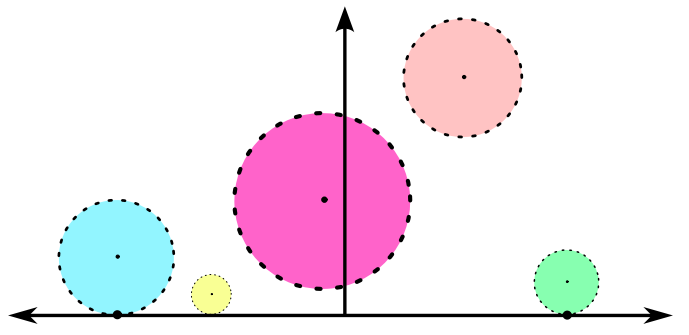
\includegraphics[width=0.5\linewidth]{pics/openSetsinMoorePlane.png}
    \caption{Open Sets in the Moore Plane}
\end{figure}

\begin{topology}[Arithmetic Progression Topology]\label{topology:z-arith-topology}
    Define a topology on $\mathbb{Z}$ denoted by $\mathbb{Z}_{arith}$ with basis:
    \begin{align*}
        B = \{ a \mathbb{Z} + b \mid a, b \in \mathbb{Z}, a \neq 0 \}.
    \end{align*}
\end{topology}

\subsection{Topologies on the Three-Element set}

Topologies on the three-element set can be useful examples. There are nine distinct topologies (up to homeomorphsim), with representatives of each equivalence class by:
\begin{align*}\label{topology:3-element-topology}
    \mathcal{T} &= \{ \emptyset, \{ a\}, \{b\}, \{c \}, \{a, b \}, \{b, c \}, \{a, c \}, \{a, b, c \} \}, \\
    \mathcal{T} &= \{ \emptyset, \{b \}, \{a, b \}, \{b, c \}, \{a, b, c \} \}, \\ 
    \mathcal{T} &= \{ \emptyset, \{b \}, \{a \}, \{a, b \}, \{b, c \}, \{a, b, c \} \}, \\
    \mathcal{T} &= \{ \emptyset, \{a, b\}, \{a, b, c \} \}, \\
    \mathcal{T} &= \{ \emptyset, \{a \}, \{a, b\}, \{a, b, c \} \}, \\
    \mathcal{T} &= \{ \emptyset, \{ b \}, \{a, b\}, \{a, b, c \} \}, \\
    \mathcal{T} &= \{ \emptyset, \{a \}, \{ b \}, \{a, b\}, \{a, b, c \} \}, \\
    \mathcal{T} &= \{ \emptyset, \{c \}, \{a, b\}, \{a, b, c \} \} \\
    \mathcal{T} &= \{ \emptyset, \{c\}, \{a, b, c \} \}. \\
    \mathcal{T} &= \{ \emptyset, \{a, b, c \} \}.
\end{align*}

\newpage
\section{Key Theorems and Lemmas}

We will not list every theorem here prove (as many are essentially trivialities) and we will not provide proofs for things already in the notes. 

\subsection{Sets, Relations, Functions, and Order}

\subsubsection{Notes 01}

\subsubsection{Notes 02}

\subsubsection{Notes 03}

\begin{theorem}\label{theorem:induced-maps-commute-w-operations}
    Given a map $f: A \to B$:
    \begin{enumerate}
        \item Prove that the induced map $\bar{f} : \mathcal{P}(A) \to \mathcal{P}(B)$ preserves order (under subsets) and commutes with union.
        \item Prove that the induced map $\bar{f^{-1}}: \mathcal{P}(B) \to \mathcal{P}(A)$ preserves order and commutes with union, intersection, and complement.
    \end{enumerate}
\end{theorem}

\begin{theorem}\label{theorem:bijection-power-set-two-point-function-space}
    There is a bijection $\mathcal{P}(A) \to 2^{A}$ with $2 = \{0, 1\}$.
\end{theorem}

\subsubsection{Notes 04}

\begin{proposition}\label{proposition:uniqueness-of-suprema}
    Given a poset $A$, if $A' \subset A$ has a supremum, it is unique.
\end{proposition}

\begin{proposition}\label{proposition:complete-lattice}
    For any set $A$, the power set $\mathcal{P}(A)$ with $\le$ by inclusion is a complete lattice.
\end{proposition}

\begin{theorem}\label{theorem:order-preserving-maps-have-fixed-pts}
    Every order-preserving map of $A \to A$ for $A$ a complete lattice has a fixed point.
\end{theorem}

\begin{corollary}\label{corollary:fixed-point-decomposition-of-order-preserving-maps}
    Let $f: A \to B$ and $g: B \to A$ as follows. Then we can split $A$ and $B$ by:
    \begin{itemize}
        \item There exist $A_1, A_2$ disjoint with $A_1 \cup A_2 = A$.
        \item There exist $B_1, B_2$ disjoint with $B_1 \cup B_2 = B$.
        \item $\overline{f}(A_1) = B_1$, $\overline{g}(B_2) = A_{2}$.
    \end{itemize}
\end{corollary}

\begin{theorem}[Schroeder-Bernstein]\label{theorem:schroeder-bernstein}
    If $|A| \le |B|$ and $|B| \le |A|$, then $|A| = |B|$.
\end{theorem}

\begin{proposition}\label{proposition:total-order-of-cardinalities}
    All cardinalities are comparable.
\end{proposition}

\begin{proof}
    Given sets $A, B$, use the Well-Ordering Principle to well-order $A$ and $B$, then apply $\Cref{theorem:well-ordered-set-isomorphisms}$ to conclude either $|A| = |B|$, $|A| \le |B|$ ($A$ is an initial segment of $B$), or $|B| \le |A|$ ($B$ is an initial segment of $A$). 
\end{proof}

\begin{proposition}\label{proposition:from-surjection-get-injection}
    If there is a surjection $A \to B$, there exists an injection $B \to A$ (requires choice).
\end{proposition}

\begin{proof}
    If there is a surjection $A \to B$, for each $b \in B$, take $f^{-1}(B)$. Define a map $B \to A$ using choice to select exactly one element from each $f^{-1}(B)$.
\end{proof}

\begin{theorem}[Cantor]\label{theorem:diagonalization}
    For any set $A$, $|A| < |\mathcal{P}(A)|$.
\end{theorem}

\begin{proposition}\label{proposition:subset-of-countable-countable}
    Any subset of a countable set is countable.
\end{proposition}

\begin{theorem}\label{theorem:countable-union-of-countable-is-countable}
    A countable union of countable sets is countable.
\end{theorem}

\begin{proposition}\label{proposition:product-of-countables-is-countable}
    A product of countable sets is countable.
\end{proposition}

\begin{theorem}\label{theorem:R-uncountable}
    $\mathbb{R}$ is uncountable.
\end{theorem}

\subsubsection{Notes 05}

\begin{lemma}\label{lemma:order-preserving-injections}
    Let $f: A \to A$ be an order-preserving injection of a well-ordered set into itself. Prove that $a \le f(a)$ for all $a \in A$.
\end{lemma}

\begin{proof}
    Take the set $X = \{ x \mid x > f(x) \}$, assume it is nonempty. Let $x_0$ be the least element of this set (guaranteed by well-ordering of $A$). Then $x_0 > f(x_0)$, hence since $x_0$ was minimal, $f(x_0) \notin X$, so $f(x_0) \le f(f(x_0))$. But since $x_0 > f(x_0)$, order-preservation tells us $f(x_0) > f(f(x_0))$, a contradiction. So $X$ must be empty as desired.
\end{proof}

\begin{corollary}\label{corollary:well-ordered-not-iso-initial-segment}
    Prove that a well-ordered set is not order-isomorphic to any of its initial segments.
\end{corollary}

\begin{proof}
    We show something stronger - there is no order-preserving injection $A$ to an initial segment of $A$. Assume there exists an order injection $f: A \to S_{a}$ where $S_{a}$ is the initial segment $S_{a} = \{ a' \in A \mid a' < a \}$. 
    
    Then, we know $f(a) \ge a$ by the prior problem. But, $y \in S_{a}$ has the property that $y < a$, so for $y = f(a)$, we simultaenously have $f(a) < a$ and $f(a) \ge a$, a contradiction. Hence no such map can exist.
\end{proof}

\begin{theorem}\label{theorem:well-ordered-set-isomorphisms}
    Let $A, B$ be well-ordered sets. Then exactly one of the following is true:
    \begin{enumerate}
        \item $A$ is order-isomorphic to $B$.
        \item $A$ is order-isomorphic to an initial segment of $B$.
        \item $B$ is order-isomorphic to an initial segment of $A$.
    \end{enumerate}
\end{theorem}


\begin{theorem}[Zermello's Theorem/Choice Equivalents]\label{theorem:choice-equivalents}
    The following are equivalent:
    \begin{enumerate}
        \item (Axiom of Choice) If $A$ is a set of nonempty sets, there is always a function $f: A \to \bigcup A$ such that $f(a) \in a$ for all $a \in A$.
        \item (Well-Ordering Property, Zermelo's Postulate) Every set can be well-ordered.
        \item (Haussdorff Maximum Principle) Every poset $A$ has a maximal totally ordered subset $S$ (in that there exists an $S \subset A$ totally ordered with no $T$ with $S \subset T \subset A$ such that $T$ is totally ordered).
        \item (Zorn's lemma) If $A$ is a poset in which every totally ordered subset has an upper bound, then $A$ has a maximal element (meaning there is no larger element). 
    \end{enumerate}
\end{theorem}

\begin{proposition}\label{proposition:existence-minimal-uncountable-set}
    There exists a minimal uncountable well-ordered set $S$ with a last element $\Omega$ such that if $a < \Omega$, the initial segment of $a$ is countable. 
\end{proposition}

\begin{proof}
    See HW02.
\end{proof}

\newpage
\subsection{Topological Spaces}

\subsubsection{Notes 06}

\begin{proposition}\label{proposition:balls-around-A-open}
    For any subset $A$ of a metric space $M$ and any $\epsilon > 0$, $B(A, \epsilon)$ is open.
\end{proposition}

\begin{proof}
    See HW02.
\end{proof}

\begin{proposition}\label{proposition:closure-in-metric-space}
    In a metric space $M$,
    \begin{align*}
        \overline{A} = \{ x \in M \mid d(x, A) = 0 \}.
    \end{align*}
\end{proposition}

\begin{proof}
    See HW.
\end{proof}

\begin{proposition}\label{proposition:closed-metric-sets-G-sigma}
    In a metric space $M$, a closed subset is $G$-$\sigma$, meaning it is a countable intersection of open sets. 
\end{proposition}

\begin{proof}
    See HW03.
\end{proof}

\subsubsection{Notes 07}

\begin{theorem}[Continuity in Metric Spaces]\label{theorem:continuity-equiv-metric-general}
    The definition of continuity in metric spaces \Cref{def:continuity-metric} is equivalent to the definition of continuity for general topological spaces \Cref{def:continuity-general} when we let the topological space be the one induced by the metric.
\end{theorem}

\begin{lemma}\label{lemma:closed-sets-characterize-a-topology}
    A collection of closed sets $X$ closed under the operations of finite union and arbitrary intersection characterizes a topology.
\end{lemma}

\begin{theorem}[Kuratowski-Closure-Axioms]\label{theorem:kuratowski-closure-axioms}
    The closure operation $A \to \overline{A}$ satisfies:
    \begin{enumerate}
        \item $A \subset \overline{A}$.
        \item $\overline{\overline{A}} = \overline{A}$.
        \item $\overline{(A \cup B)} = \overline{A} \cup \overline{B}$.
        \item $\overline{\emptyset} = \emptyset$.
    \end{enumerate}
    Conversely, given any function $f:\mathcal{P}(X) \to \mathcal{P}(X)$ by $A \to \overline{A}$ satisfying these, there is a unique topology equal to $X - \Im(f)$.
\end{theorem}

\begin{theorem}[Dual Kuratowski Interior Axioms]\label{theorem:dual-kuratowski-interior-axioms}
    The interior operation $A \to A^{\circ}$ satisfies:
    \begin{enumerate}
        \item $A^{\circ} \subset A$.
        \item $(A^{\circ})^{\circ} = A^{\circ}$.
        \item $(A \cap B)^{\circ} = A^{\circ} \cap B^{\circ}$
        \item $X^{\circ} = X$.
    \end{enumerate}
    Conversely,any $f$ acting by $A \to A^{\circ}$ in this way defines a topology by $\Im(f)$.
\end{theorem}

\begin{theorem}[Decomposition by a set $A$]\label{theorem:interior-exterior-boundary-decomposition}
    Given any $A \subset X$, we have:
    \begin{align*}
        X = (X - \overline{A}) \bigsqcup \delta A \bigsqcup A^{\circ}
    \end{align*}
    with $(X - \overline{A}), A^{\circ}$ open.
\end{theorem}

\subsubsection{Notes 08}

\begin{lemma}[Characterization of Open Sets with Neighborhoods]\label{lemma:characterization-of-opens-by-neighborhoods}
    $U \subset X$ is open if and only if for each $x \in U$ there is a neighborhood $N_{x}$ of $x$ contained in $U$, i.e $U$ is a neighborhood of all $x \in U$.
\end{lemma}

\begin{theorem}[Hausdorff Neighborhood Axioms]\label{theorem:haussdorff-neighborhood-axioms}
    Let $\mathcal{N}(x)$ denote the set of neighborhoods of a point $x \in X$. Then:
    \begin{enumerate}
        \item If If $N \in \mathcal{N}(x)$ then $x \in N$.
        \item $N \in \mathcal{N}(x)$ and $N \subset M$, then $M \in \mathcal{N}(x)$.
        \item The set $\mathcal{N}(x)$ is closed under finite intersections.
        \item If $N \in \mathcal{N}(x)$, there exists some $N' \in \mathcal{N}(x)$ such that $N'$ is a neighborhood of all $y \in N'$, that is, $y \in N'$ implies $N \in \mathcal{N}(y)$.
    \end{enumerate}
    Conversely, given a nonempty collection $\mathcal{N}(x)$ of neighborhoods of $x$ for each $x \in X$ satisfying the above axioms, there is a unique topology for which $\mathcal{N}(x)$ is the collection of neighborhoods of $x$.
\end{theorem}

The topology is defined by $U$ is open if for all $y \in U$, $U \in \mathcal{N}(y)$.

\begin{theorem}
    Every metrizable space is first countable.
\end{theorem}

\begin{proof}
    Take the balls $B(x, \frac{1}{n})$. These form a countable neighborhood basis at $x$, as for any open set $U$ with $x \in U$, there exists a disc $B(x, \epsilon)$ with $x \in B(x, \epsilon) \subset U$, and then finding a $\frac{1}{n}$ with $\frac{1}{n} < \epsilon$ shows $x \in B(x, \frac{1}{n}) \subset B(x, \epsilon) \subset U$, so we are done.
\end{proof}

\begin{theorem}\label{neighborhood}
    Let $\mathcal{B}(x)$ be a neighborhood basis at $X$. Then:
    \begin{enumerate}
        \item Given $U \in \mathcal{B}(x)$, we know $x \in U$.
        \item If $U-1, U_2 \in \mathcal{B}(x)$, then there exists $V \in \mathcal{B}(x)$ with $V \subset U_1 \cap U_2$.
        \item If $U \in \mathcal{B}(x)$, there exists $V \subset U$ such that for $y \in V$, $V \in \mathcal{N}(y)$.
    \end{enumerate}
\end{theorem}

The topology is defined by $U$ is open if for $x \in U$, there is $B \in \mathcal{B}(x)$ with $x \in B \subset U$.

\begin{theorem}[Topology Generated by a Basis]\label{theorem:topology-generated-by-a-basis}
    Given $\mathcal{B}$ a set of subsets of $X$, $\mathcal{B}$ is a basis for the topology generated by $\mathcal{B}$ if and only if $\bigcup \mathcal{B} = X$ and the intersection of two elements of $\mathcal{B}$ is a union of elements of $\mathcal{B}$.
\end{theorem}

\begin{proof}
    If $\mathcal{B}$ is a base for the topology generated by itself, the result is obvious. Conversely, if $\mathcal{B}$ has the given properties, let $\mathcal{T}$ be the set of all unions of sets of $\mathcal{B}$. This is closed under unions (and finite intersections) with the given properties (namely the condition $\bigcup \mathcal{B} = X$ is necessary to include the empty intersection), every set of $\mathcal{B}$ is open, and no smaller topology satisfies the given conditions.
\end{proof}

\begin{lemma}\label{lemma:neighborhood-condition-for-closures}
    Let $x \in X$, $A \subset X$. Then $x \in \overline{A}$ if and only if every neighborhood of $x$ meets $A$.
\end{lemma}

\begin{corollary}\label{corollary:boundary-in-terms-of-neighborhoods}
    We have:
    \begin{align*}
        \delta A= \{ x \in X \mid \text{ every neighborhood of $x$ meets both } A, X-A \}.
    \end{align*}
\end{corollary}

\begin{proof}
    We know $\delta A = \overline{A} - A^{\circ}$. Since $x \in \overline{A}$, $x$ must meet $A$. Since $x \notin A^{\circ}$, $x \in X-A^{\circ}$, but as $X-A^{\circ} = \overline{X-A}$ (which is not hard to show), $x \in \overline{X-A}$, so we see neighborhoods $x$ must also meet $X-A$.
\end{proof}

\begin{corollary}\label{corollary:closure-is-accumulation-pts-with-all-of-A}
    The closure $\overline{A}$ has $\overline{A} = A \bigcup A'$.
\end{corollary}

\subsubsection{Notes 09}

\begin{lemma}\label{lemma:composition-continuous}
    If $f: X \to Y$ continuous at $x_0$, $g: Y \to Z$ continuous at $y_0 = f(x_0)$, then $g \circ f : X \to Z$ is continuous at $x_0$.
\end{lemma}

\begin{theorem}[Characterizations of Continuity]\label{theorem:characterization-of-continuity}
    Given a function $f: X \to Y$, the following are equivalent:
    \begin{enumerate}
        \item $f$ is continuous
        \item $f(\overline{A}) \subset \overline{f(A)}$ for $A \subset X$.
        \item If $B$ is closed in $Y$, then $f^{-1}(B)$ is closed in $X$.
        \item If $B$ is open in $Y$, $f^{-1}(B)$ is open in $X$.
    \end{enumerate}
\end{theorem}

\begin{proposition}[Homeomorphisms and Topologies]\label{proposition:homeomorphisms-correspond-to-bijections-of-topology}
    Given topological spaces $(X, \mathcal{T})$, $(Y, \mathcal{S})$, a continuous bijection $f: X \to Y$ is a homeomorphism if and only if the induced map $f^{*}: \mathcal{S} \to \mathcal{T}$ by $V \to f^{-1}(V)$ is a bijection.
\end{proposition}

\begin{proof}
    If $V \to f^{-1}(V)$ is a bijection of $\mathcal{S}$ and $\mathcal{T}$, we know we can write every open set $U \in X$ as $f^{-1}(V)$ for some unique $V \in Y$. Then the map $f^{-1}: Y \to X$ by $A \to f^{-1}(U)$ is a homeomorphism as any open set $U \subset X$ will be $f^{-1}(V)$ of some $V$, hence the preimage $(f^{-1})^{-1}(U)$ will be $f(f^{-1}(V)) = V$ open, showing $f^{-1}$. 

    Conversely if $f^{-1}: Y \to X$ is a continuous bijection (we already know it's a bijection), we know for each $U \in X$, $(f^{-1})^{-1}(U) = V$ for some unique $V$ open in $Y$, but this gives $f(U) = V$, and since $f$ is a bijection we conclude $U = f(V^{-1})$, so each open in $X$ is a unique preimage of an open in $V$, i.e $f^*: \mathcal{S} \to \mathcal{T}$ is a bijection. 
\end{proof}

\begin{lemma}\label{lemma:condition-for-continuity-by-subbases}
    If $f: X \to Y$ with $\mathcal{C}$ a subbasis for $Y$, $f$ is continuous if and only if $f^{-1}(c)$ is open for each $c \in \mathcal{C}$.
\end{lemma}



\newpage
\section{Important Counterexamples}

\subsection{Continuous Maps}

\begin{example}[Continuous Bijection NOT a Homeomorphism]
    Consider the identity map $\id: \mathbb{R}_{LL} \to \mathbb{R}$. Since the lower limit topology is strictly finer than the standard topology, the preimage of an open set (hence a neighborhood) is certainly open (containing a neighborhood), but the reverse is not true since we have open sets in the Sorgenfrey line not open in $\mathbb{R}$.
\end{example}


\subsection{First and Second Countability}

\begin{example}[First but not Second Countable]\label{counterexample:first-not-second-countable-space}
    Consider the \Cref{topology:discrete-topology} with $X$ uncountable. Since every set is open, any open set $U \supset x$ will contain the open set $\{ x \}$ as a subset, so $\{ x \}$ will be in every neighborhood and this will be a countable neighborhood basis. 

    However, we certainly cannot have a countable basis for the whole space, as each singleton is open, so such a basis would include every singleton (otherwise there would be no nonempty open set $U \in \mathcal{B}$ with $U \subset \{ x \} $ for all $X$), making the basis uncountable.
\end{example}

Notice this shows actually that even a metric space is not necessarily second countable, although metric spaces ARE first countable, as the discrete topology is induced by a metric. 

\begin{example}[Non-First-Countable Space]\label{counterexample:non-first-countable-space}
    Apply the \Cref{topology:cofinite-topology} on $\mathbb{R}$, and consider a point $\{ 0 \}$. We will show there is no countable neighborhood basis for this point. If there existed such a countable neighborhood basis, we would have open sets $V_i = X - C_i$ (with $C_i$ finite) such that for any open $V$ (we can specialize to the case of open $V$ for general neighborhoods by taking $V^{\circ}$) with $\{ 0 \} \subset V$, there is some $V_i$ with $0 \notin V_i \subset V$. But, such a $V$ would be $X-C$ with $C$ finite, meaning $\{ 0 \} \notin x-C_i \subset X-C$, i.e $0 \in C \subset C_i$, so we want a set of $C_i$ for every $C$ finite and containing $0$, there is a finite $C_i$ containing it.  
    
    But since the $C_i$ are finite, the union of the $C_i$ is countable, and for a set above, we would then see $0 \in C \subset \bigcup C_i$ for all $C$, hence the union of the $C_i$ must be all of $\mathbb{R}$ (since we could take $C = \{a, 0 \}$ for every $a \in \mathbb{R}$ implying $a \in \bigcup C_i$. But this is then impossible since if the $C_i$ are finite their countable union is countable. 
\end{example}

\subsection{Separation Axioms}

\subsection{Metrizability}

\newpage
\section{Table of Topological Properties versus Topology}

\begin{center}
\begin{table}[htp!]
\begin{tabular}{|l|l|l|l|l|l|l|l|l|l|l|l|l|l|l|}
\hline
          & $\mathbb{R}_{std}$ & $\mathbb{R}_{std}^{n}$                                                         & $\mathbb{R}_{par}^{n}$ & $X_{ind}$ & $X_{dis}$   & $X_{cof}$  & $X_{coc}$ & $\mathbb{R}_{LL}$ & $\mathbb{R}_{00}$ & $\mathbb{R}_{har}$ & $H_{bub}$    & $\mathbb{Z}_{ari}$ & $2^{X}$      & $X_{order}$  \\ \hline
$T_1$     & $\checkmark$       & $\checkmark$                                                                   & $\checkmark$           & $\times$     & $\checkmark$ & $\checkmark$ & $\checkmark$  & $\checkmark$      & $\checkmark$      & $\checkmark$       & $\checkmark$ & $\checkmark$         & $\checkmark$ & $\checkmark$ \\ \hline
Hau. & $\checkmark$       & $\checkmark$                                                                   & $\checkmark$           & $\times$     & $\checkmark$ & $\times$     & $\times$      & $\checkmark$      & $\times$          & $\checkmark$       & $\checkmark$ & $\checkmark$         & $\checkmark$ & $\checkmark$ \\ \hline
Reg.   & $\checkmark$       & $\checkmark$                                                                   & $\checkmark$           & $\times$     & $\checkmark$ & $\times$     & $\times$      & $\checkmark$      & $\times$          & $\times$           & $\checkmark$ & $\checkmark$         & $\checkmark$ & $\checkmark$ \\ \hline
Nor.    & $\checkmark$       & $\checkmark$                                                                   & $\checkmark$           & $\times$     & $\checkmark$ & $\times$     & $\times$      & $\checkmark$      & $\times$          & $\times$           & $\times$     & $\checkmark$         & $\checkmark$ & $\checkmark$ \\ \hline
1-Ct & $\checkmark$       & $\checkmark$                                                                   & $\checkmark$           & $\checkmark$ & $\checkmark$ & $\times$     & $\times$      & $\checkmark$      & $\checkmark$      & $\checkmark$       & $\checkmark$ & $\checkmark$         & $\times$     & $\times$     \\ \hline
2-Ct & $\checkmark$       & \hyperref[property:rn-std-second-countable]{$\checkmark$} & $\times$               & $\checkmark$ & $\times$     & $\times$     & $\times$      & $\times$          & $\checkmark$      & $\checkmark$       & $\times$     & $\checkmark$         & $\times$     & $\times$     \\ \hline
Sep.    & $\checkmark$       & $\checkmark$                                                                   & $\times$               & $\checkmark$ & $\times$     & $\checkmark$ & $\checkmark$  & $\checkmark$      & $\checkmark$      & $\checkmark$       & $\checkmark$ & $\checkmark$         & $\times$     & $\times$     \\ \cline{15-15} 
\end{tabular}
\end{table}
\end{center}

Things I do not have arguments for SOMEWHERE:
- $\mathbb{R}^{n}_{par}$ a metric space NOT second countable.
- separation axioms for order topology
- $2^{X}$ is normal 
- $H_{bub}$ normal (cant explain argument properly)

Order topology fails using minimal uncountable well-ordered set (write up somewhere?)

Here, topologies that can be applied to an arbitrary $X$ are marked false if for SOME $X$ they fail.

\newpage 
\section{Proofs of Interesting Facts}

\subsection{$\mathbb{R}_{std}^n$}

\begin{theorem}\label{property:rn-metrizable}
    
\end{theorem}

\begin{theorem}\label{property:rn-first-countable}
    
\end{theorem}

\begin{theorem}\label{property:rn-std-second-countable}
    The topological space $\mathbb{R}^{n}_{std}$ is second countable. 
\end{theorem}

\begin{proof}
    We claim $\mathbb{R}_{std}^{n}$ has a basis by the collection of open balls with rational centers and rational radii, which is certainly countable.

    We need to show for an arbitrary basic open set $U = B(r, \epsilon)$ and $p\ in U$, there exists $B_p$ a ball with rational center and rational radii with:
    \begin{align*}
        p \in B_p \subset U  
    \end{align*}
    Given any $p$ in the ball $B(r, \epsilon)$, we know $d(p, r) < \epsilon$. Let $\alpha = d(p, r) > 0$. 
    
    By density of $\mathbb{Q}$, we claim can find some rational point $q$ with $d(p, q) < \frac{\epsilon - \alpha}{2}$. We know $p$ has coordinates $(p_1, ..., p_n)$ and same with $r = (r_1, ..., r_n)$, so we know:
    \begin{align*}
        \sqrt{(r_1-p_1)^2 + ... + (r_n-p_n)^2} = \alpha
    \end{align*}
    Then finding a $q_i$ with $q_i - p_i < \frac{1}{\sqrt{n}} \frac{(\epsilon - \alpha)^2}{4}$ (which we can do by density of $\mathbb{Q}$ in $\mathbb{R}$ and the fact that $\epsilon - \alpha > 0$), we can find $q_i$ such th)at:
    \begin{align*}
        \sqrt{(r_1-p_1)^2 + ... + (r_n-p_n)^2} < \sqrt{\frac{1}{n}\frac{(\epsilon - \alpha)^2}{4} + ... + \frac{1}{n}\frac{(\epsilon - \alpha)^2}{4}} = \frac{\epsilon - \alpha}{2}.
    \end{align*}
    Then, notice:
    \begin{align*}
        d(r, q) \le d(r, p) + d(p, q) < \alpha + \frac{\epsilon - \alpha}{2} = \frac{\epsilon + \alpha}{2}. 
    \end{align*}

    We now claim the ball $B(q, s)$ for $s$ a rational number such that $d(p, q) < s < \frac{\epsilon - \alpha}{2}$ (which we can again find via density) satisfies:
    \begin{align*}
        p \in B(q, s) \subset B(r, \epsilon).
    \end{align*}
    Certainly since $d(p, q) < s$, $p \in B(q, s)$. If $t \in B(q, s)$, we know:
    \begin{align*}
        d(r, t) \le d(r, q) + d(q, t) < \frac{\epsilon + \alpha}{2} + \frac{\epsilon-\alpha}{2} = \epsilon,
    \end{align*}
    thus $t \in B(r, \epsilon)$ as desired.
\end{proof}



\end{document}